\chapter{Identity Binding Multi Issuer Multi Credential Anonymous Credentials}\label{chap3}

\section{Introduction}\label{sec:mimc}
Anonymous credential systems enable users to prove statements about their attributes while preserving privacy, evolving from single-issuer designs (e.g., Idemix~\cite{camenisch_design_2002}) to meet complex, real-world demands. Unlike Chapter 2's single-issuer $\ABC$ system, we address the problem \emph{how can users privately combine credentials from multiple, mutually distrusting issuers to prove they belong to the same identity, without revealing it?}

Consider a user proving they hold (1) a government-issued ID confirming residency, (2) an employer credential verifying income, and (3) a training certificate—all tied to one identity, without linking them via a public identifier. Alternatively, in content credentialing, a user might present images signed by different devices (e.g., cameras) to a journal, proving they share an account while selectively disclosing metadata. Existing approaches fall short: attribute-based signatures lack aggregation~\cite{cimato_signature_2003}, aggregate signatures assume a single issuer \cite{goos_short_2001, hutchison_short_2004} or limit revocation flexibility~\cite{hebant_traceable_nodate}, and generic zkSNARKs, while expressive, incur high computational costs~\cite{rosenberg_zk-creds_2022}. CanDID~\cite{maram2021candid} binds credentials via a consistent name, but this offers weaker security against malicious issuers and their system lacks issuer-privacy for internal identifiers. ZKcreds~\cite{rosenberg_zk-creds_2022} uses a zkSNARK-based join gadget for multi-credential proofs, yet its proof computation scales poorly, especially for multiple credentials. Our Multi-Issuer Multi-Credential Anonymous Credential system (MIMC-ABC) overcomes these limitations with a secure, efficient solution.

MIMC-ABC employs position-binding commitments and zero-knowledge proofs to cryptographically bind credentials from distinct issuers to a single, private identifier, ensuring anonymity and unforgeability even against colluding adversaries. We formalize a security model for multi-issuer identity binding, define the identity binding property, and provide rigorous proofs of its guarantees. Our comprehensive attack taxonomy—covering forgery, predicate manipulation, and binding attacks—demonstrates robustness, while a scaling analysis shows security holds as issuers and credentials grow. Performance evaluations reveal that privacy-preserving multi-issuer verification, though roughly 3× slower than non-private baselines (e.g., 18.67ms vs. 6.77ms for 4 credentials), remains efficient for practical use.

\subsection{Contributions}
This chapter advances the state of anonymous credentials with:
\begin{itemize}
    \item A formalized multi-issuer security model with an identity binding property, ensuring credentials from distinct issuers provably belong to the same user without compromising anonymity
    \item Security proofs showing resilience as the number of issuers and credentials increases.
    \item A performance evaluation methodology comparing non-private, private single-issuer (with batch verification), and private multi-issuer scenarios, quantifying privacy’s overhead.
\end{itemize}

\todonote{must update the identity binding show}

\begin{figure}
    \centering
    \begin{tikzpicture}[
        box/.style={draw, rounded corners=2pt, minimum width=6cm, minimum height=8.5cm},
        smallbox/.style={draw, rounded corners=2pt, fill=gray!10, minimum width=5cm, minimum height=2.5cm},
        verifierbox/.style={draw, rounded corners=2pt, minimum width=4cm, minimum height=4cm},
        showbox/.style={draw, rounded corners=2pt, fill=gray!10, minimum width=4.7cm, minimum height=2.5cm},
        thick
    ]
    
    % Digital Credential Wallet
    \node[box] (wallet) at (0,0) {};
    \node[anchor=south, font=\bfseries] at ($(wallet.north) + (0,0.3)$) {Credential Wallet};
    
    % Master Credential
    \node[smallbox] (master) at (0,2.75) {};
    \node[anchor=north, font=\small\bfseries] at ($(master.north) + (0,-0.3)$) {Master Credential};
    
    \node[anchor=north west, font=\small, align=left] at ($(master.north west) + (0.5,-0.7)$) {
        \texttt{id : 12345}, \\
        \texttt{ctx : "passport"}, \\
        \texttt{exp : "10/11/2026"}, \\
        \texttt{k : 54321}
    };
    
    % Driver License Credential
    \node[smallbox] (driver) at (0,0) {};
    \node[anchor=north, font=\small\bfseries] at ($(driver.north) + (0,-0.3)$) {Driver License};
    
    \node[anchor=north west, font=\small, align=left] at ($(driver.north west) + (0.5,-0.7)$) {
        \texttt{id : 12345}, \\
        \texttt{ctx : "DMV"}, \\
        \texttt{exp : "10/11/2028"}
    };

    % Bank Statement Credential
    \node[smallbox] (bank) at (0,-2.75) {};
    \node[anchor=north, font=\small\bfseries] at ($(bank.north) + (0,-0.3)$) {Bank Statement};
    
    \node[anchor=north west, font=\small, align=left] at ($(bank.north west) + (0.5,-0.7)$) {
        \texttt{id : 12345}, \\
        \texttt{ctx : "bankstatement"}, \\
        \texttt{date : "10/11/2027"}, \\
        \texttt{bal : "10,000,000"}
    };
    
    % % Add dividing lines between credentials in wallet
    % \draw[dashed, thick] ($(wallet.west) + (0.2,1.4)$) -- ($(wallet.east) + (-0.2,1.4)$);
    % \draw[dashed, thick] ($(wallet.west) + (0.2,-1.4)$) -- ($(wallet.east) + (-0.2,-1.4)$);
    
    % Credential Show in the middle (replacing Nullifier Generation)
    \node[showbox] (show) at (6.5,0) {};
    \node[anchor=north, font=\bfseries] at ($(show.north) + (0,-0.3)$) {Identity Binding Show};
    
    % Add the deterministic nullifier algorithm with section reference
    \node[font=\small, align=center] at ($(show.north) + (0,-1.3)$) {Sec: \ref{subsec:deterministic-nullifier} $y = g^{1/(k + \text{"DMV"})}$};
    
    % Add the probabilistic nullifier algorithm with section reference
    \node[font=\small, align=center] at ($(show.north) + (0,-2.0)$) {Sec: \ref{sec-probabilistic-nullifier} $\cm_y = g_1^{1/(k + \text{"DMV"})}g^{\usk_3}$};
    
    % Verifier box (replacing the two boxes on the right)
    \node[verifierbox] (verifier) at (12,0) {};
    \node[anchor=north, font=\bfseries] at ($(verifier.north) + (0,-0.3)$) {Verifier};
    
    % Draw contents for the verifier box
    \node[font=\small, align=center] at ($(verifier.north) + (0,-2.0)$) {
        Validates credentials\\
        Checks signatures\\
        Verifies proofs
    };

    % Arrows from wallet edge to credential show
    \draw[->, thick] ($(wallet.east) + (0,2.75)$) -- ($(show.west) + (0,0.5)$);
    \draw[->, thick] ($(wallet.east) + (0,0)$) -- (show.west);
    \draw[->, thick] ($(wallet.east) + (0,-2.75)$) -- ($(show.west) + (0,-0.5)$);
    
    % % Arrows from credentials to the credential show
    % \draw[->, thick] (master.east) -- ++(0.5,0) -- ($(show.west) + (0,0.5)$);
    % \draw[->, thick] (driver.east) -- (show.west);
    % \draw[->, thick] (bank.east) -- ++(0.5,0) -- ($(show.west) + (0,-0.5)$);
    
    % Arrow from credential show to verifier
    \draw[->, thick] (show.east) -- (verifier.west);
    
    \end{tikzpicture}
    \caption[Credential Showing Scheme]{A credential showing scheme for privacy-preserving protocols, illustrated with a credential hierarchy binding multiple credentials (passport, driver's license, bank statement) to enable secure and privacy-preserving presentation to verifiers.}
    \label{fig:credential-show-revised}
\end{figure}




\section{System Model and Definitions}

Our Multi-Issuer Multi-Credential Anonymous Credential (MIMC-ABC) system extends the single-issuer Attribute-Based Anonymous Credential (ABC) framework from Chapter 2 to support credentials from multiple, mutually distrusting issuers, bound to a single identity. The ABC system (Section 2.4) uses a variant of rerandomizable Pointcheval-Sanders signatures~\cite{sako_short_2016} and position-binding Pedersen commitments~\cite{tomescu_utt_2022} to enable expressive predicate proofs over attributes. MIMC-ABC builds on this by introducing multi-issuer key generation and a cryptographic identity binding mechanism, ensuring all credentials verifiably belong to the same user without revealing their identity.

\subsection{MIMC-ABC Syntax}

A MIMC-ABC system consists of the following probabilistic polynomial-time (PPT) algorithms, parameterized by a security parameter $\lambda$ and attribute vector length $\ell$:

\begin{definition}[MIMC-ABC]
    \begin{itemize}
    \item $\mathsf{Setup}(1^\lambda) \to \mathsf{pp}$: Outputs public parameters $\mathsf{pp}$, including a bilinear group $\BG = (\G_1, \G_2, \G_T, e, g, \tilde{g}, p)$ as in Section 2.1.
    
    \item $\mathsf{OrgKeyGen}(\mathsf{pp}, \ell, j) \to (\mathsf{osk}_j, \mathsf{opk}_j)$: For issuer $j$, takes $\mathsf{pp}$ and $\ell$, outputs a keypair $(\mathsf{osk}_j, \mathsf{opk}_j)$ using the signature scheme from Section 2.3.

    \item $(\mathsf{Obtain}(\attrs, \{\mathsf{opk}_j\}_j, \mathsf{aux}), \mathsf{Issue}(\mathsf{osk}_j, \mathsf{cm}, \mathsf{aux})) \to (\mathsf{cred}_j, \bot)$: An interactive protocol between a user and issuer $j$. The user inputs an attribute vector $\attrs = [\id, \ctx_j, \exp_j]$, where $\id$ is a unique identifier, $\ctx_j$ is the issuer-specific context, and $\attrs_j$ are attributes. The user samples $\usk_j \sample \Z_p$, commits as $\mathsf{cm} \gets \mathsf{CM.Com}(\attrs; \usk_j)$, and proves its opening (Section 2.4.3). The issuer signs $\mathsf{cm}$ with $\mathsf{osk}_j$, outputting $\mathsf{cred}_j = (\sigma_j, \mathsf{cm})$ to the user and $\bot$ to itself.

    \item $(\mathsf{Show}(\{\mathsf{cred}_j\}_j, \{\usk_j\}_j, \phi), \mathsf{Verify}(\{\mathsf{cred}_j'\}_j, \pi)) \to \{0,1\}$: An interactive protocol between a user and verifier. The user inputs a set of credentials $\{\mathsf{cred}_j\}_j$ from (optionally) distinct issuers, rerandomizes each $(\sigma_j, \mathsf{cm})$ to $(\sigma_j', \mathsf{cm}')$, and computes a proof $\pi$ that $\phi(\{\attrs_j\}_j) = 1$ and all $\id$ values match, using $\Sigma$-protocols (Section 2.4.3). The verifier checks the proof and rerandomized credentials against $\{\mathsf{opk}_j\}_j$, outputting 1 if valid, 0 otherwise.
\end{itemize}
\end{definition}


\subsection{Security Properties}

MIMC-ABC inherits the core security properties from the ABC system—correctness, unforgeability, and anonymity (Section 2.5)—and adds identity binding for the multi-issuer setting:

\begin{itemize}
    \item \textbf{Correctness}: An honest user with valid credentials from multiple issuers can generate a proof for any predicate $\phi$ their attributes satisfy, including same-identity constraints, which verifies with probability $1 - \negl(\lambda)$.
    
    \item \textbf{Unforgeability}: No PPT adversary can produce a valid proof for a predicate $\phi$ they cannot legitimately satisfy, including forging credentials or mixing credentials from different identities, except with negligible probability.
    
    \item \textbf{Anonymity}: Proofs reveal only that $\phi$ is satisfied, not the user’s identity or credential details, even if all issuers and the verifier collude.
    
    \item \textbf{Identity Binding}: When $\phi$ requires all credentials to share the same $\id$, no PPT adversary can produce a valid proof using credentials with differing $\id$ values, except with negligible probability.
\end{itemize}

\subsection{Identity Binding Property}

We formalize identity binding as a distinct security property for multi-issuer systems:



\begin{definition}[Identity Binding]
A MIMC-ABC system satisfies identity binding if for all PPT adversaries $\mathcal{A}$, there exists a negligible function $\mathsf{negl}$ such that:
\[
\Pr\left[
\begin{array}{l}
    \mathsf{pp} \gets \mathsf{Setup}(1^\lambda) \\
    \{(\mathsf{osk}_j, \mathsf{opk}_j)\}_j \gets \mathsf{OrgKeyGen}(\mathsf{pp}, \ell) \\
    (\{\mathsf{cred}_j'\}_j, \phi^*, \pi^*) \gets \mathcal{A}^{\mathcal{O}}(\{\mathsf{opk}_j\}_j)
\end{array}
: \begin{array}{l}
    \mathsf{Verify}(\{\mathsf{cred}_j'\}_j, \phi^*, \pi^*) = 1 \land \\
    \phi^* \text{ requires } \forall j, \id_j = \id \land \\
    \exists j, k: \id_j \neq \id_k
\end{array}
\right] \leq \mathsf{negl}(\lambda)
\]
where $\mathcal{O}$ includes oracles for honest user creation, corruption, credential issuance, and proof generation (adapted from Section 2.5).
\end{definition}

This ensures that credentials presented together must share a single, private $\id$, enforced via position-binding commitments and zero-knowledge proofs, as detailed in Section 3.













\section{Construction}

Our MIMC-ABC system constructs credentials as rerandomizable Pointcheval-Sanders signatures from \cite{tomescu_utt_2022} over position-binding Pedersen commitments, extending the single-issuer ABC system (Section 2.4) to bind credentials from multiple issuers to a shared, private identifier. We leverage the algebraic structure of these primitives and $\Sigma$-protocols to prove credential validity and identity consistency efficiently, supporting predicates over an arbitrary number of attributes.

\subsection{Intuition}

Each credential from issuer $j$ commits to an attribute vector $\attrs_j = [\id, \ctx_j, \exp_j]$, where $\id$ is a unique, user-chosen identifier, $\ctx_j$ denotes the credential’s context (e.g., "passport"), and $\exp_j$ is an expiration date. The vector can extend to additional attributes as needed (e.g., income, degree, date of birth). 

Each credential from issuer $j$ commits to an attribute vector $\attrs_j = [\id, \ctx_j, \exp_j]$, where $\id$ is a unique, user-chosen identifier, $\ctx_j$ denotes the credential’s context (e.g., "passport"), and $\exp_j$ is an expiration date. The vector can extend to additional attributes as needed (e.g., income, degree). Issuance is flexible: the user privately commits to $\mathsf{cm}_1 = \mathsf{CM.Com}([\id, 0, 0]; \usk_j)$ with randomness $\usk_j$ and proves its opening and proves it commits to zero's in positions 2, 3, while issuer $j$ commits to $\mathsf{cm}_2 = \mathsf{CM.Com}([0, \ctx_j, \exp_j]; 0)$ and homomorphically combines them into $\mathsf{cm}_j = \mathsf{cm}_1 \cdot \mathsf{cm}_2 = \mathsf{CM.Com}([\id, \ctx_j, \exp_j]; \usk_j)$, signing it. Alternatively, the user can commit to all attributes privately, and the issuer signs directly, supporting both fully private and issuer-driven scenarios (e.g., credential oracles like DECO~\cite{zhang_deco_2020}). To present credentials, the user rerandomizes each signature and commitment, then proves in zero-knowledge that: (1) all signatures are valid under their respective issuer keys, and (2) all commitments share the same $\id$, satisfying a predicate $\phi$.

For example, consider a user with credentials from three issuers ($j = 1, 2, 3$): a passport, driver’s license, and university degree, each with the same $\id = 12345$ (Figure~\ref{fig:three-creds}). The user rerandomizes each pair $(\sigma_j, \mathsf{cm}_j)$ to $(\sigma_j', \mathsf{cm}_j')$ and proves they meet a policy, e.g., $\phi = (\ctx_1 = \text{"passport"} \land \exp_1 > \text{today} \land \ctx_2 = \text{"dmv"} \land \ctx_3 \in \mathcal{D})$, where $\mathcal{D}$ is a set of accredited universities.

\begin{figure}[h]
    \centering
    \begin{pchstack}[boxed, center, space=4em]
        \begin{pcvstack}
            \procedure[space=auto]{Passport ($j=1$)}{
                \id: 12345, \\
                \ctx_1: "passport", \\
                \exp_1: "10/11/2026"
            }
        \end{pcvstack}
        \pcvspace
        \begin{pcvstack}
            \procedure[space=auto]{Driver’s License ($j=2$)}{
                \id: 12345, \\
                \ctx_2: "dmv", \\
                \exp_2: "05/01/2027"
            }
        \end{pcvstack}
        \pcvspace
        \begin{pcvstack}
            \procedure[space=auto]{University Degree ($j=3$)}{
                \id: 12345, \\
                \ctx_3: "usyd-bcompsc", \\
                \exp_3: "12/31/2024"
            }
        \end{pcvstack}
    \end{pchstack}
    \caption{Example credentials from three issuers, sharing $\id = 12345$. Additional attributes (e.g., degree type) can be included.}
    \label{fig:three-creds}
\end{figure}

\subsection{Construction Details}

The MIMC-ABC system operates as follows, reusing primitives from Chapter 2 (Sections 2.3, 2.4):

\begin{itemize}
    \item $\mathsf{Setup}(1^\lambda)$: Generates $\mathsf{pp}$ with bilinear group $\BG = (\G_1, \G_2, \G_T, e, g, \tilde{g}, p)$ and commitment generators $(g_1, g_2, g_3, \tilde{g}_1, \tilde{g}_2, \tilde{g}_3)$ for $\ell = 3$, extensible to more attributes.
    
    \item $\mathsf{OrgKeyGen}(\mathsf{pp}, \ell, j)$: Issuer $j$ runs $\mathsf{RS.KeyGen}$ (Section 2.3) to produce $(\mathsf{osk}_j, \mathsf{opk}_j)$, with $\mathsf{opk}_j = (\vk_j, \ck_j)$.

    \item $\mathsf{Obtain}$ and $\mathsf{Issue}$: The user commits $\mathsf{cm}_j = \mathsf{CM.Com}([\id, \ctx_j, \exp_j]; \usk_j)$, proves its opening via $\pircom$ (Section 2.4.3), and sends it to issuer $j$. Issuer $j$ signs it as $\sigma_j = \mathsf{RS.Sign}(\mathsf{cm}_j, \mathsf{osk}_j)$, returning $\mathsf{cred}_j = (\sigma_j, \mathsf{cm}_j)$. The user retains $\usk_j$.

    \item $\mathsf{Show}$ and $\mathsf{Verify}$: For credentials $\{\mathsf{cred}_j\}_j$, the user:
        \begin{enumerate}
            \item Rerandomizes: $\mathsf{cm}_j' = \mathsf{CM.Rerand}(\mathsf{cm}_j, \Delta_{r_j})$, $\sigma_j' = \mathsf{RS.Rerand}(\sigma_j, \Delta_{r_j}, \Delta_{u_j})$.
            \item Proves via $\Sigma$-protocol:
                \[
                \mathcal{R}_\phi =\left\{ 
                \begin{array}{l} 
                (\{\mathsf{cm}_j', \sigma_j'\}_j, (\id, \{\ctx_j, \exp_j, \usk_j + \Delta_{r_j}\}_j)) \\
                \end{array} 
                \middle|
                \begin{array}{l}
                \forall j: \mathsf{RS.Ver}(\sigma_j', \mathsf{cm}_j', \vk_j) = 1 \land \\
                \mathsf{cm}_j' = g_1^\id g_2^{\ctx_j} g_3^{\exp_j} g^{\usk_j + \Delta_{r_j}} \land \\
                \phi(\{\ctx_j, \exp_j\}_j) = 1
                \end{array} 
                \right\}
                \]
        \end{enumerate}
        The verifier checks $\pi$ and $\{\mathsf{opk}_j\}_j$, accepting if valid.
\end{itemize}



\subsection{Identity Binding Mechanism}

Identity binding relies on the position-binding property of Pedersen commitments (Section 2.2). The $\Sigma$-protocol proves that all $\mathsf{cm}_j'$ share the same $\id$ in the first position ($g_1^\id$), using an equality proof across commitments:
\[
\rid = \zkpok \left\{ 
\begin{array}{l} 
(\{\mathsf{cm}_j'\}_j, (\id, \{\usk_j', \ctx_j, \exp_j\}_j)) \\
\end{array} 
\middle|
\begin{array}{l}
\forall j: \mathsf{cm}_j' = g_1^\id g_2^{\ctx_j} g_3^{\exp_j} g^{\usk_j'}
\end{array} 
\right\}
\]
The position-binding assumption (SDLP, Section 2.1) ensures an adversary cannot forge commitments with different $\id$ values that appear equal, reducing security to standard cryptographic hardness.






\section{Security Analysis}

We analyze the security of MIMC-ABC against a PPT adversary controlling issuers, corrupting users, and querying oracles (adapted from Section 2.5). Our system inherits the ABC framework’s guarantees (Section 2.6) and strengthens them with identity binding for the multi-issuer setting. We prove correctness informally, then formalize unforgeability, anonymity, and identity binding, reducing security to the underlying primitives’ assumptions: EUF-CMA of the signature scheme (Section 2.3), position-binding of the commitment scheme (Section 2.2), and soundness of $\Sigma$-protocols (Section 2.4.3).

\subsection{Correctness}

An honest user with valid credentials $\{\mathsf{cred}_j\}_j$ from issuers $\{j\}$ can always generate a proof $\pi$ for a predicate $\phi$ their attributes $\{\attrs_j\}_j = \{[\id, \ctx_j, \exp_j]\}_j$ satisfy, including same-$\id$ constraints. Rerandomization ensures signatures and commitments verify under $\{\mathsf{opk}_j\}_j$, and the $\Sigma$-protocol proves $\phi$ and $\id$ equality with probability $1 - \negl(\lambda)$, following Section 2.6’s correctness argument extended to multiple issuers.

\subsection{Unforgeability}

\begin{theorem}[Unforgeability]
MIMC-ABC is unforgeable if the rerandomizable signature scheme is EUF-CMA secure, the Pedersen commitment scheme is position-binding, and the $\Sigma$-protocol is sound. For any PPT adversary $\mathcal{A}$, $\Adv^{\mathsf{UNF}}_{\MIMCABC, \mathcal{A}}(\lambda) \leq \negl(\lambda)$.
\end{theorem}

\begin{proof}[Sketch]
We reduce unforgeability to three cases, adapting Section 2.6’s ABC proof:
\begin{enumerate}
    \item \textbf{Forged Signature}: If $\mathcal{A}$ outputs a valid $\mathsf{cred}_j' = (\sigma_j', \mathsf{cm}_j')$ not issued by any $\mathsf{osk}_j$, we extract $\sigma_j'$ as an EUF-CMA forgery.
    \item \textbf{Predicate Misuse}: If $\mathcal{A}$ uses valid credentials but proves a false $\phi^*$ (e.g., $\exp_j < \text{today}$ when $\exp_j > \text{today}$), the $\Sigma$-protocol’s special soundness lets us extract a witness contradicting the original attributes, breaking position-binding.
    \item \textbf{Identity Mixing}: If $\mathcal{A}$ combines credentials with different $\id$ values yet proves same-$\id$, we extract two openings of some $\mathsf{cm}_j'$ (e.g., $g_1^{\id_1}$ vs. $g_1^{\id_2}$), breaking position-binding.
\end{enumerate}
A reduction $\mathcal{B}$ simulates the game (Section 2.5), embedding EUF-CMA and position-binding challenges into $\{\mathsf{opk}_j\}_j$ and $\mathsf{cm}_j$. Any forgery violates one assumption, bounding $\mathcal{A}$’s advantage by $\negl(\lambda)$.
\end{proof}

\subsection{Anonymity}

\begin{theorem}[Anonymity]
MIMC-ABC is anonymous, even against colluding issuers, if the signature scheme’s rerandomization is indistinguishable, the commitment scheme is hiding, and the $\Sigma$-protocol is zero-knowledge. For any PPT adversary $\mathcal{A}$, $\Adv^{\mathsf{ANON}}_{\MIMCABC, \mathcal{A}}(\lambda) \leq \negl(\lambda)$.
\end{theorem}

\begin{proof}[Sketch]
We use a hybrid argument, extending Section 2.6’s ABC anonymity proof:
\begin{itemize}
    \item \textbf{Hybrid 0}: Real game with user $i_b$’s credentials $\{\mathsf{cred}_j\}_j$, rerandomized and proven via $\mathsf{Show}$.
    \item \textbf{Hybrid 1}: Replace $\pi$ with a simulated proof using the $\Sigma$-protocol’s zero-knowledge simulator.
\end{itemize}
The hiding property of Pedersen commitments ensures $\mathsf{cm}_j'$ is uniform, signature rerandomization makes $\sigma_j'$ indistinguishable from fresh signatures, and the simulated $\pi$ hides $i_b$, even if all issuers share $\{\mathsf{osk}_j\}_j$. The advantage is negligible as hybrids are computationally indistinguishable.
\end{proof}

\subsection{Identity Binding}

\begin{theorem}[Identity Binding]
MIMC-ABC satisfies identity binding under the SDLP assumption (Section 2.1). For any PPT adversary $\mathcal{A}$ mixing credentials with distinct $\id$ values, $\Adv^{\mathsf{BIND}}_{\MIMCABC, \mathcal{A}}(\lambda) \leq n \cdot m \cdot \Adv^{\mathsf{SDLP}}(\lambda) + \negl(\lambda)$, where $n$ is the number of issuers and $m$ is credentials per user.
\end{theorem}

\begin{proof}[Sketch]
If $\mathcal{A}$ outputs $\{\mathsf{cred}_j'\}_j$, $\phi^*$ requiring same $\id$, and $\pi^*$ verifying despite $\id_j \neq \id_k$ for some $j, k$, the $\Sigma$-protocol’s special soundness extracts witnesses from $\pi^*$. For each $\mathsf{cm}_j' = g_1^{\id_j} g_2^{\ctx_j} g_3^{\exp_j} g^{\usk_j'}$, we get $\id_j$, and differing $\id$ values imply two openings of some $\mathsf{cm}_j'$ at position 1 (e.g., $g_1^{\id_1}$ vs. $g_1^{\id_2}$). A reduction $\mathcal{B}$ embeds an SDLP challenge $(g^x, \tilde{g}^x)$ into $g_1, \tilde{g}_1$, solving $x$ with probability $1/(n \cdot m)$ per credential, yielding the bound.
\end{proof}

\subsection{Security Scaling}

The identity binding advantage scales linearly with $n$ and $m$, reflecting the number of opportunities to break position-binding. This graceful degradation ensures MIMC-ABC remains secure as the system grows, a key advantage over prior multi-issuer schemes lacking formal binding guarantees.

\section{Identity Binding Application: Improving KYC/AML Identity Verification}

\todonote{Sam to do}
Speak about the KYC/AML process and why identity binding is necessary


\section{Performance Evaluation}

We evaluate MIMC-ABC to quantify the overhead of privacy-preserving multi-issuer credential verification, comparing it against non-private and single-issuer baselines. Unlike prior multi-issuer systems (e.g., CanDID~\cite{maram_candid_2020}, ZKcreds~\cite{rosenberg_zk-creds_2022}), MIMC-ABC balances strong identity binding with practical efficiency, leveraging our signature optimization \ref{rerandsig_g2}. Our benchmarks focus on verification time—the critical path in authentication—across three scenarios: non-private, private single-issuer with batch signature aggregation, and private multi-issuer.

\subsection{Methodology}

We implemented MIMC-ABC using the arkworks library~\cite{arkworks_contributors_arkworks_2022} on a BLS12-381 curve (128-bit security), running on a MacBook Air M2 (16GB RAM, macOS Sequoia 15.3.2). We measure verification time for 4, 16, and 32 credentials, each with 4 attributes, averaging 100 trials (standard deviation < 5\%). Scenarios include:
\begin{enumerate}
    \item \textbf{Non-Private}: Signatures verified with batch aggregation, revealing $\attrs_j$ in the clear—a common baseline for non-anonymous systems.
    \item \textbf{Private Single-Issuer}: All credentials from one issuer, using batch verification of PS signatures (Section 2.3) and a $\Sigma$-protocol for same-$\id$ and predicate satisfaction.
    \item \textbf{Private Multi-Issuer}: Each credential from a different issuer, requiring individual signature verification and a $\Sigma$-protocol for identity binding (worst-case scenario).
\end{enumerate}




\begin{figure}
    \centering
   
    % Bottom row with 2x2 grid of smaller figures
    \begin{minipage}{0.48\textwidth}
        \centering
        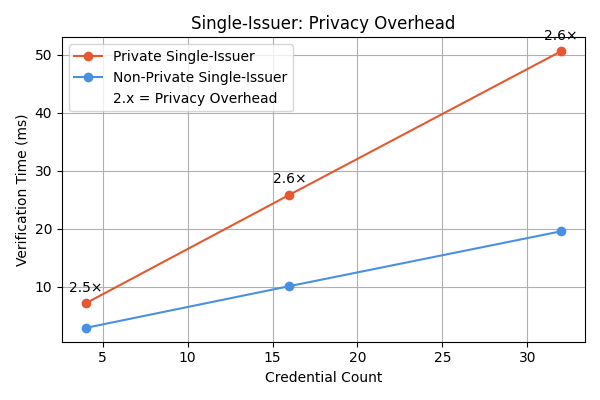
\includegraphics[width=\textwidth]{figures/chap3_single_issuer_privacy_overhead.png}
    \end{minipage}
    \hfill
    \begin{minipage}{0.48\textwidth}
        \centering
        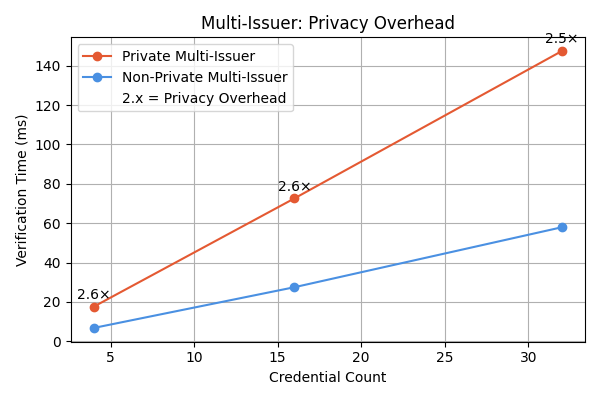
\includegraphics[width=\textwidth]{figures/chap3_multi_issuer_privacy_overhead.png}
    \end{minipage}
    
    \caption{Performance Comparison between UTT and Our Construction. We improve key operations: Verify and Show + Verify}
    \label{fig:chap3_privacy_overhead_graphs}
\end{figure}




\begin{figure}
    \centering
   
    % Bottom row with 2x2 grid of smaller figures
    \begin{minipage}{0.48\textwidth}
        \centering
        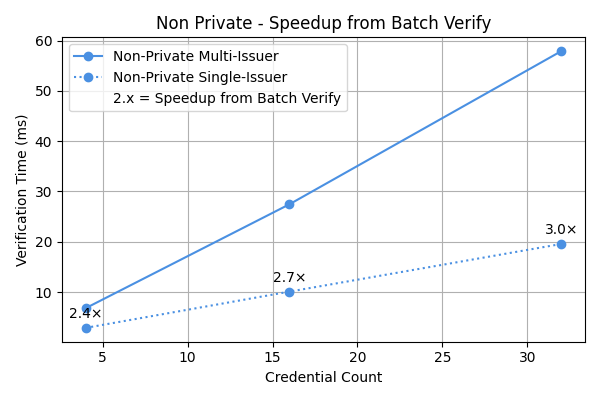
\includegraphics[width=\textwidth]{figures/chap3_nonprivate_batch_speedup.png}
    \end{minipage}
    \hfill
    \begin{minipage}{0.48\textwidth}
        \centering
        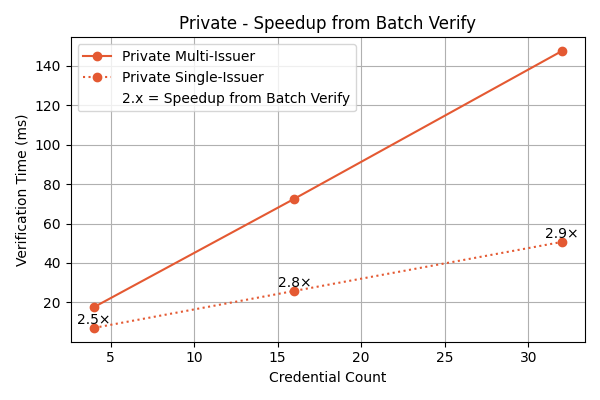
\includegraphics[width=\textwidth]{figures/chap3_private_batch_speedup.png}
    \end{minipage}
    
    \caption{Performance Comparison between UTT and Our Construction. We improve key operations: Verify and Show + Verify}
    \label{fig:chap3_batch_verify_improvements}
\end{figure}




\begin{table}[ht]
\centering
\caption{Varying Credential Count, Set Attribute Number (4) (time in ms)}
\label{tab:performance-credentialscaling-chap3}
\begin{tabular}{l@{\hspace{1em}}r@{\hspace{0.5em}}r@{\hspace{0.5em}}r@{\hspace{0.5em}}r@{\hspace{1em}}r}
\toprule
\textbf{Scenario} & \multicolumn{3}{c}{\textbf{Verify (ms)}} & \textbf{Overhead Avg.} & \textbf{Notes} \\
\cmidrule(lr){2-4}
& \textbf{4 Creds} & \textbf{16 Creds} & \textbf{32 Creds} &  & \\
\midrule
Non-Private Single-Issuer & 2.87 & 10.08 & 19.55 & -- & Cleartext, batched \\
Private Single-Issuer & 7.11 & 25.85 & 50.64 & 2.5× & Batch verification \\
\midrule
Non-Private Multi-Issuer & 6.79 & 27.45 & 57.88 & -- & Cleartext, distinct issuers \\
Private Multi-Issuer & 17.65 & 72.57 & 147.35 & 2.6× & Worst-case, distinct issuers \\
\bottomrule
\end{tabular}
\end{table}


\begin{table}[ht]
\centering
\caption{Varying Attribute Count, Set Credential Count (4) (time in ms)}
\label{tab:performance-attributescaling-chap3}
\begin{tabular}{l@{\hspace{1em}}r@{\hspace{0.5em}}r@{\hspace{0.5em}}r@{\hspace{0.5em}}r@{\hspace{1em}}r}
\toprule
\textbf{Scenario} & \multicolumn{3}{c}{\textbf{Verify (ms)}} & \textbf{Overhead} & \textbf{Notes} \\
\cmidrule(lr){2-4}
& \textbf{4 Attrs} & \textbf{16 Attrs} & \textbf{32 Attrs} & \textbf{(32 vs. 4 Attrs)} & \\
\midrule
Non-Private Single-Issuer & 2.87 & 2.85 & 2.87 & 1.0× & Cleartext, batched \\
Private Single-Issuer & 7.11 & 7.28 & 8.03 & 1.1× & Batch verification \\
\midrule
Non-Private Multi-Issuer & 6.79 & 6.77 & 6.81 & 1.0× & Cleartext, distinct issuers \\
Private Multi-Issuer & 17.65 & 18.67 & 19.89 & 1.1× & Worst-case, distinct issuers \\
\bottomrule
\end{tabular}
\end{table}


\subsection{Discussion}

Table~\ref{tab:performance-credentialscaling-chap3} highlights the impact of credential scaling. Non-private single-issuer verification benefits from batch aggregation, scaling near-linearly (2.87ms to 19.55ms). Private single-issuer verification adds a consistent 2.5× overhead across credential counts, remaining efficient due to batching. Non-private multi-issuer verification scales from 6.79ms to 57.88ms, reflecting the cost of individual signature checks. Private multi-issuer verification, at 17.65ms to 147.35ms, incurs a 2.6× overhead at 4 credentials, increasing slightly to 2.5× at 32 credentials, as the lack of batching dominates.

Table~\ref{tab:performance-attributescaling-chap3} examines attribute scaling for 4 credentials. Increasing attributes from 4 to 32 has minimal impact on non-private scenarios (e.g., 2.87ms to 2.87ms for single-issuer, 6.79ms to 6.81ms for multi-issuer), as attribute processing is lightweight without privacy. For private scenarios, the overhead is modest: private single-issuer grows from 7.11ms to 8.03ms (1.1×), and private multi-issuer from 17.65ms to 19.89ms (1.1×). This small increase reflects the efficiency of $\Sigma$-protocols in handling additional attributes, a key advantage of MIMC-ABC over zkSNARK-based systems like ZKcreds, which scale poorly with attribute complexity.

In practice, users often hold credentials from a mix of issuers—some repeated, some unique. For example, a user might present two government credentials (batchable) and two from distinct employers, blending single- and multi-issuer efficiency. The worst-case multi-issuer scenario is thus unlikely in full, making MIMC-ABC’s average-case performance even more competitive. 
% How does attribute verification scale in zk-creds? 